

The proposed autoscaling system scales a web application in response to change in throughput at fixed intervals, which we denote by reconfiguration intervals of 10 minutes. This system is able to provision the right amount and type of vm instances for minimizing the number of SLA violations while keeping the operational cost adapted to the customer requirements. Vertical and horizontal scaling actions can be applicable to satisfy the service demand. This architecture has the following key components:

\vspace{2mm}

\textbf{Predictor: } Inspired by~\cite{wolski_network_1999}, the Predictor component takes the monitoring data as input and uses different time-series analysis techniques to predict the future service demand for the next time interval. To provide accurate forecasting measures, this component utilizes the technique that exhibited the lowest cumulative error measure during the previous monitoring window. By doing so, the Predictor is able to adapt the predictions to the current type of workload. This component supports five distinct statistical models that fits four types of workload: \emph{(1)} \emph{Linear Regression} for linear trends~\cite{muppala_regression-based_2012}, \emph{(2)} \emph{Auto Regression Moving Average} (ARMA) for linear with small oscillations~\cite{roy_efficient_2011},\emph{(3)} \emph{Exponential Smoothing} for daily and seasonal~\cite{exponential_smoothing2010}, and \emph{(4)} \emph{Autoregression} and \emph{Vector Autoregression} for correlated trends~\cite{chandra_dynamic_2003,vector_autoregression_2006}. 

\vspace{2mm}

\textbf{Profiler: } To choose a scaling plan, provisioning systems have to know the limitations of the different server configurations when running an application. The definition of profiles for each instance's type improves the accuracy of the scaling actions in heterogeneous cloud infrastructures. Thus, the Profiler component calculates the optimal throughput of each type of provisioned vm instance using profiling techniques.

% without any server instrumentation.

\vspace{2mm}

\textbf{Dynamic load balancer: } In order to adapt our system to the heterogeneity of requests and cloud resources, this component dynamically assign weights to the backend servers to proportionally distribute the incoming traffic based on the performance characteristics of each backend. As an example, a server with four cores is able to process a higher number of requests so its weight has to a be greater than a server with only one core.

\vspace{2mm}

\textbf{Scaler:} This component contains the central intelligence of our autoscaling system. As illustrated in Figure~\ref{autoScalingSys}, Scaler uses the Predictor and Profiler components to find the optimal provisioning strategy that fulfills a pre-established SLO (Service Level Objective). Furthermore, this component constantly analyzes the behavior of each provisioned vm triggering the Dynamic load balancer component when need it.

\begin{figure}[htb]
  \begin{center}
    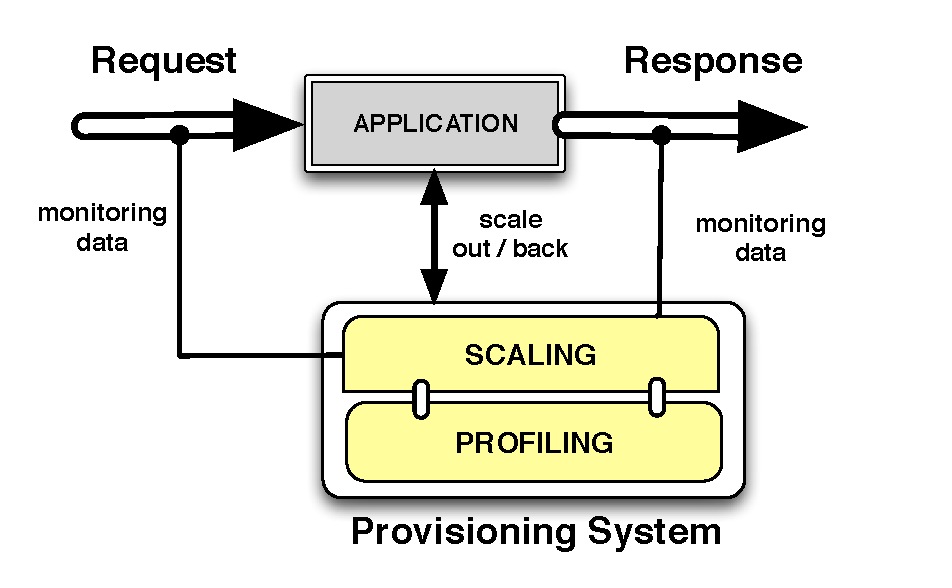
\includegraphics[width=.85\linewidth]{images/monitoringSchema}
  \end{center}
\vspace{-5mm}
  \caption{Autoscaling system.}
  \label{autoScalingSys}
\end{figure}

%In the following we ..

%\subsection{Online profiling of allocated instances\label{profiling}}
\subsection{Online instance profiling\label{profiling}}

Regarding the resource heterogeneity of cloud infrastructures, a sensitivity analysis of the allocated resources is crucial to provide accurate scaling decisions. Accordingly, online profiling-based techniques~\cite{kaviani_profiling-as--service:_2011} have recently emerged as a solution to  estimate the resource's throughput under a certain workload. Traditionally, this technique replicates at runtime a server hosting an application, with a new server with profiling instrumentation that analyzes the performance behavior of a specific resource under a fixed percentage of the incoming traffic~\cite{jiangThesis,dejavu2012}. The use of fixed workloads to calculate the maximum throughput of a resource do not necessary imply the definition of more accurate profiles. A reason seems to be the lack of ideal performance isolation in cloud infrastructures which affects to the precision of the definitions, and consequently reduces the accuracy of the decisions. Furthermore, setting a profiling environment, in a heterogeneous cloud infrastructure, requires as many additional resources as number of available server configurations. Even though the use of online-profiling techniques is still under study, the configuration of a parallel environment and the heterogeneity of the cloud resources are the major drawbacks for its adoption. These techniques increase the operational cost and do not necessarily improve the accuracy of the scaling decisions.

%Even though the use of online-profiling techniques is still under study, the configuration of a parallel %environment and the limited accuracy of its scaling decisions are the major drawbacks for its %adoption.

As a consequence, we designed a novel online profiling technique that gives an estimation of the maximum throughput of each allocated instance's type without need for additional resources or parallel environments. To do that, the Profiler component use the provisioned resources for the analysis and estimation of the computing capacity of each available hardware configuration.

\begin{algorithm}
{\scriptsize
\SetAlgoLined
\SetInd{0mm}{2mm}
\KwData{ \\Service Level Objective, \emph{slo} \\ List of allocated instance types, \emph{inst\_types} \\ Compute units per \emph{inst\_type}, \emph{compute\_units$_{inst}$}}

\KwResult{Instances performance classification}

\While{ allocated instances to profile}{
\BlankLine
Collect profiling data of \emph{inst\_type}: \emph{req\_rate, cpu\_usage and resp\_time}\;

\While{ profiling data to smooth}{  \label{alg:smooth}
//Perform smoothing percentiles technique \;
\If{ \emph{resp\_time}$_i$ $>$ (slo * 0.25) and \emph{resp\_time}$_i$ $<=$ (slo * 0.75)}{ 
	\If{ \emph{req\_rate}$_i$ $>$ 0 and \emph{cpu\_usage}$_i$ $<$ 75}{ 
		\hspace{3mm} Add \emph{cpu\_usage$_i$} to cpu\_usage\_data\;
		\hspace{3mm} Add \emph{req\_rate$_i$} to req\_rate\_data\;
		\hspace{3mm} Add \emph{resp\_time$_i$} to resp\_time\_data\;
}
}
} \label{alg:endSmooth}
\BlankLine
Initialize instance capacity \emph{CPU speed$_{inst}$} to 0 \;
\uIf{ \emph{resp\_time\_data}, \emph{cpu\_usage\_data}, \emph{req\_rate\_data}  \textbf{not empty}}{
Calculate average of \emph{cpu\_usage\_data}, \emph{CPU$_{inst}$} \;
Calculate average of \emph{req\_rate\_data}, \emph{Num\_requests$_{inst}$} \;
\BlankLine
\emph{CPU speed$_{inst}$} = $\dfrac{\emph{CPU$_{inst}$} } {\emph{Num\_requests$_{inst}$} }$  \;
\BlankLine
Store instance computing capacity, \emph{CPU speed$_{inst}$} \;
}
\Else{ 
	Use historic value of \emph{CPU speed$_{inst}$} for \emph{inst\_type}\;
}
\BlankLine
Classify \emph{inst\_type} based on its computing capacity \;
\If{ CPU speed$_{inst}$ = 0 }{
Use \emph{compute\_units$_{inst}$} of \emph{inst\_type} to rank \emph{inst\_type} \;
}
\Else{ 
Use new value of \emph{CPU speed$_{inst}$} to rank \emph{inst\_type} \;
}
}
}
\caption{Instance profiling algorithm}
\label{profilingAlg}
\end{algorithm}

As detailed in Algorithm~\ref{profilingAlg}, once the Scaler component decides to trigger a scaling action, the Profiler component estimates the throughput of the allocated instances according the following steps:

\begin{enumerate}
\item Collect the latest hour of monitoring data from each instance's type. This profiling data contains information about monitoring metrics such as the request rate, cpu usage and response time, which provide enough feedback for the definition of instance profiles. 

\item Perform a smoothing technique over the profiling data of each instance to remove the noise generated by traffic spikes. As pointed out in~\cite{gandhi_hybrid_2012}, when hosting web applications sudden changes in the workload, interference due to virtualization or OS activities may affect the precision of the profiling process. Hence, we decided to smooth the profiling data during the latest hour (or older if there is not enough data) to identify the performance capacity of one instance. In particular, the Profiler extracts the smoothed 75th and 25th percentiles from the response times below the SLO and 75th percentile from the cpu usage data-points. (See Lines \ref{alg:smooth}-\ref{alg:endSmooth}). This mechanism allows to identify the maximum ideal throughput of each instance while enforcing the performance requirements and avoiding CPU saturation. (based on the Amazon EC2 recommendation CPU usage < 75 )

As an example in Figure~\ref{fig:vm_performance}, we show the profiling data and percentiles for one "m1.small" (left) and one "c1.medium" (right) EC2 instance types during one hour. The gray areas represent the ranges of response times and cpu usage comprised by the percentiles. Red circles contain all data points that will be used to calculate the maximum ideal throughput of one instance. As we mentioned above, some data points are excluded as they identify periods of time on which resources suffered from under-utilization or over-utilization (denoted by white areas). Furthermore, as shown in Figure~\ref{fig:vm_performance} (left), a short number of data points are comprised between the percentiles for the "m1.small" instance. Its poor hardware configuration makes this type of instance more vulnerable to sudden changes in the workload.

%and three red circles highlight several data-points on which the performance of the instance was optimal while enforcing the %SLO.

%\begin{figure*}[htb]
%	\begin{minipage}[b]{0.5\linewidth}
%		\includegraphics[height=4.5cm]{images/vm_performance_resp_smallEC2Remark.pdf}		%\includegraphics[height=4.5cm]{images/vm_performance_cpu_smallEC2Remark.pdf}
%		\vspace{-4mm}
%	\end{minipage}
%	\hfill
%	\begin{minipage}[b]{0.5\linewidth}
%		\includegraphics[height=4.5cm]{images/vm_performance_resp_c1mediumRemark.pdf}		%\includegraphics[height=4.5cm]{images/vm_performance_cpu_c1mediumRemark.pdf}
%		\vspace{-4mm}
%	\end{minipage}
%\caption{Profiling data and percentiles of m1.small and c1.medium EC2 instances.}
%\label{fig:vm_performance}
%\end{figure*}

\begin{figure*}[htb]
	\begin{minipage}[b]{0.45\linewidth}
		\includegraphics[height=8.5cm]{images/idealSmallRemark.pdf}	
		\vspace{-4mm}
	\end{minipage}
	\hfill
	\begin{minipage}[b]{0.45\linewidth}
		\includegraphics[height=8cm]{images/idealc1MediumRemark.pdf}
		\vspace{-4mm}
	\end{minipage}
\caption{Profiling data and percentiles of m1.small and c1.medium EC2 instances.}
\label{fig:vm_performance}
\end{figure*}

\item Classify the different instance types depending on its computing capacity. Using the profiling smoothed data of each instance type, the Profiler computes a factor, named \emph{CPU speed}, as the number of clocks required to process a request (clocks/request), where \emph{CPU$_{inst}$} represents the average of cpu usage and \emph{Num\_requests$_{inst}$} the average of request rate, as illustrated in the next Equation~\ref{cpu_speed}:

\begin{equation}\label{cpu_speed}
\begin{split}
CPU speed_{inst} = \dfrac{  CPU_{inst} } {Num\_requests_{inst} } 
\end{split}
\end{equation}


The \emph{CPU speed$_{inst}$} factor gives an estimation of the ideal performance capacity of one instance when processing the current workload. Based on the value of this factor per-instance, the \emph{Profiler} classifies the different instances based on its computing capacity when running an application. The resulting classification gives an interesting feedback to the Scaler component, which is now able to identify the limitations of the instances, and consequently to choose an optimal scaling plan. Initially, there are not instance profiles due to the lack of monitoring data, thereby the Scaler uses the number of compute units per instance as a priori classification of their performance capacities. Note that, this work only consider the compute units, but memory or bandwidth can be also taken into account to classify the instances.

\end{enumerate}

This profiling process allows to define a profile per instance type, thus facilitating the selection of an appropriate scaling plan that satisfies the QoS requirements. As such, the accuracy of the scaling decisions can be improved independently of factors such as performance isolation in clouds or request heterogeneity.


\subsection{The scaling decision maker}

The Scaler component is the central governance of this autoscaling system, and thereby is the responsible of triggering any scaling decision.

%% Threshold fixed by the user

\subsubsection{Time-series smoothing}

When minimizing the SLA violations, a precise analysis of the monitoring data is crucial to improve the accuracy of the scaling decisions. It allows to identify the resource requirements from the current workload type. This analyisis has even more importance when hosting web applications (e.g. Wikipedia, Amazon) that need to provide high availability and performance to their clients. Moreover, the workload heterogeneity of this sites requires a meticulous analysis of every monitoring data-point to reduce at the maximum the number of SLO violations. 

\begin{figure}[htb]
	\begin{minipage}[b]{0.49\linewidth}
		\includegraphics[width=4cm,height=3cm]{images/data2007/proxy_outputAvg.pdf}	
		\vspace{-4mm}
	\end{minipage}
	\hfill
	\begin{minipage}[b]{0.49\linewidth}
		\includegraphics[width=4cm,height=3cm]{images/data2007/proxy_outputWMA.pdf}
		\vspace{-4mm}
	\end{minipage}
\caption{Response times for a trace: Average vs extended WMA.}
\label{fig:data_analysis}
\end{figure}

To obtain precise information (response times) that reflects the performance behavior of an application, we decided to extend a known smoothing technique called \emph{Weighted Moving Average} (WMA). This technique is widely used in resource provisioning systems instead of others such as the median, average or moving average. Using our extension of WMA, it first associated weights in an increasing order giving more importance to the latest monitoring data; and second it doubles the original weight value of each data-point that exceeds the performance requirements (response time). By doing so, the Scaler analyzes the monitoring data giving special importance to the data points on which SLO violations have occurred, and thereby being able to detect and avoid the maximum number of violations. As an example, Figure~\ref{fig:data_analysis} shows how several SLO violantions are omitted when analyzing the monitoring data using an average analytical method (left) than when using our version of WMA (right).

\subsubsection{Definition of a reactive threshold}

\fixme{Perhaps, you may want to omit this subsection, as it is more related to When to provision than How to provision ?}

Initially, the user defines several performance requirements that will be utilized by the Scaler to trigger scaling actions. As we mentioned, these QoS goals are previously specified in the Service Level Objective (SLO). In particual, when hosting web applications, these performance requirements are usually related to the maximum processing time needed to serve any request (response times). Regarding SLO fulfillment the majority of resource provisioning system aims to maintain the processing time as closer as possible to the performance requirements. However, this operation can become a problem, as provisioning systems are vulnerable to temporal traffic oscillations causing SLO violations.

Therefore, and based on the requirements, the Scaler defines a reactive threshold that will enable in advance to react against any traffic oscillation minimizing the number of SLO violations or period of time under-utilization of the provisioned resources. As shown in Figure~\ref{threshold}, this reactive threshold specifies one upper and lower boundaries creating two head-rooms between them and the performance requirements pre-defined by the user (for the response time). In the future, these two boundaries could be adjusted depending on the hardware configuration of each provisioned vm, as introduced in~\cite{beloglazov_adaptive_2010}.  


\begin{figure}[htb]
  \begin{center}
    \includegraphics[width=.85\linewidth]{images/thresholdGraphic.jpg}
  \end{center}
\vspace{-5mm}
  \caption{Reactive threshold.}
  \label{threshold}
\end{figure}

\subsubsection{Vertical and horizontal scaling}

The \emph{Scaler} component supports two ways to add and remove resources to an application: vertical and horizontal scaling.
Horizontal scaling enables to create a cluster of virtual machines associated to one application whose size is dynamically adapted to the workload variations by adding or removing vmes to the cluster. This scaling technique is commonly supported for the majority of resource provisioning systems. In our system, vertical scaling enables to add or remove resources with high or less CPU or memory using \emph{service live migration}. Using this technique, the Scaler migrates the hosted service (web application) from one virtual machine to another with better hardware configuration. To reduce the degradations caused by this type of migration or by the booting time of the new machine, the Scaler checks the proper functioning of the new machine in order to release the older one.

Thus, the \emph{Scaler} evaluates whether the current performance behavior requires to trigger any of the following scaling actions:

\begin{itemize}

\item \textbf{Scale out or up:} Additional resources are provisioned if the performance behavior exceeds the upper boundary of the reactive threshold, and the \emph{Predictor} confirms that such traffic changes will remain at least during the next monitoring window (in our experiments 5min). 

\item \textbf{Scale back or down:} Resources are released if the performance behavior exceeds the lower boundary of the reactive threshold, and the \emph{Predictor} confirms that such traffic changes will remain at least during the next monitoring window.

\end{itemize}

Note that, the \emph{Predictor} component will trigger short-term forecasts operations to minimize at the maximum the number of SLA violations, as well as to keep a high level of efficiency in the predictions. 



%\begin{figure*}[htb]
%	\begin{minipage}[b]{0.3\linewidth}
%		\includegraphics[height=4.5cm]{images/prediction_conpaas_6min.eps}
%		\vspace{-4mm}
%	\end{minipage}
%	\hfill
%	\begin{minipage}[b]{0.3\linewidth}
%		\includegraphics[height=4.5cm]{images/prediction_conpaas_10min}
%		\vspace{-4mm}
%	\end{minipage}
%	\hfill
%	\begin{minipage}[b]{0.3\linewidth}
%		\includegraphics[height=4.5cm]{images/prediction_conpaas_30min}
%		\vspace{-4mm}
%	\end{minipage}
%\caption{ConPaaS Predictions, response times for 5min, 10min and 30min ahead.}
%\label{fig:vm_performance}
%\end{figure*}

\subsubsection{Scaling strategy decision-making}
The most important and challenging phase in a resource provisioning system is the selection of an appropriate scaling strategy (combination of resources) that satisfies the performance requirements with the lowest operational cost. This operation can become more laborious when running web applications, and therefore it has been barely addressed in the existing provisioning systems. Web applications are often a target of temporal traffic variations that may cause SLO violations having an impact in the user experience. Hence, the selection of an appropriate scaling plan becomes crucial to mitigate these penalties. 


To overcome this challenging phase, the Scaler takes into consideration two aspects: resource heterogeneity and user experience. Cloud infrastructures are highly heterogeneous, offering a wide range of resource combinations. On the other hand, to boost the volume of customers, the user experience appears as a mandatory requirement in web applications contrary to budget cuts that may reduce the advantage over competitors.
Based on that, the Scaler computes the cost of all the possible resource combinations how the cost incurred by its SLO fulfillment degree and the infrastructure cost. The SLO fulfillment degree indicates the vulnerability of a strategy to experience SLO violations. To refine this search process according to the final goal and adapted to the customer preferences (user experience), the Scaler provides three classes of SLA agreements in function of the type of customer. These three classes of customers namely, gold, silver and bronze minimize the SLA violations with a different infrastructure cost. Accordingly, a gold customer pays more in order to get the best service at the cost of some extra over-provisioning. A silver customer gets good availability while a bronze customer obtains a reduced, but acceptable, SLA fulfillment but with very little over-provisioning.

Prior to any resource selection, the Scaler has to measure the requirements of the current workload. To do that, it has to compute its degree of complexity taken into account the total cpu usage and request rate served by the current scaling strategy. In Equation~\ref{workload_complexity}, the \emph{$Workload_{complex}$} factor represents the complexity of the incoming traffic and includes degradations caused by operative system activities, low network performance, vm sharing or request heterogeneity. These degradations are not detected by individually analyzing the request rate and cpu usage consumed by all the resources. Thus, the \emph{$Workload_{complex}$} is computed by using the sum of the cpu usage (denoted by \emph{$CPU\_usage_{i}$}) and the performance capacity of each allocated resource. The performance capacity is calculated as the average of the request rate served by each resource (denoted by $Num\_reqs_{i}$) and its ideal throughput (denoted by $CPU speed_{inst_{i}}$). By using the ideal throughput instead of calculating the current throughput, the Scaler is able to detect how much the current workload is affecting to the ideal performance of an instance.

{\scriptsize
\begin{equation}\label{workload_complexity}
\begin{split}
Workload_{complex}  = \dfrac{ \sum_{i=1}^N CPU\_usage_{i}  }  {  \sum_{i=1}^N \bigg(  Num\_reqs_{i}  * CPU speed_{inst_{i}}   \bigg)   }
\end{split}
\end{equation}
}

Additionally, the total cpu usage ($\sum_{i=1}^N CPU\_usage_{i} $) and request rate ($\sum_{i=1}^N  Num\_reqs_{i}$) can be calculated by the Predictor component to estimate the future service demand for the next monitoring windows (in our experiments 30min). This enables to select in advance a scaling strategy that will handle future variations in the workload, and thereby reducing the operational cost. As an example in Figure~\ref{fig:forecast}, the Predictor shows the forecast values for the resource requirements during the next 30min offering an acceptable level of accuracy. 

\begin{figure}[htb]
  \begin{center}
    \includegraphics[height=5cm]{images/prediction_conpaas_30min}
  \end{center}
\vspace{-5mm}
  \caption{ConPaaS Predictor: prediction values for 30min ahead.}
  \label{fig:forecast}
\end{figure}


To decide which type of vm instances to release or add, the Scaler uses an optimal decision tree that calculates all the possible scaling strategies.  Figure~\ref{fig:scalingTree} shows three examples of scaling actions that propose three different resource combinations using EC2 instances. In the scaling decision tree, each node represents each type of vm instance offered by the cloud infrastructure. The branches define all the possible combination of resources. While the links indicate the percentage of CPU usage consumed to process the current workload when using a specific combination. Note that, CPU values provides enough feedback about the performance capacity, as it is a function of the request complexity  and number of served requests. To calculate the CPU usage consumed by each scaling strategy to process the current workload, Scaler uses the following formula~\ref{resource_combination}. 

\begin{figure}[htb]
  \begin{center}
    \includegraphics[height=5cm]{images/scalingTree}
  \end{center}
\vspace{-5mm}
  \caption{Decision tree: scaling actions using EC2 instances.}
  \label{fig:scalingTree}
\end{figure}



%To calculate the different combinations of VM instances that enforce the performance requirements, we used the next


{\scriptsize
\begin{equation}\label{resource_combination}
\begin{split}
CPU_{strategy} = \dfrac{ \sum_{i=1}^n \bigg( \bigg( \dfrac{ Num\_reqs_{total} * Workload_{complex} }  {N}  \bigg) * CPU speed_{inst_{i}} \bigg) }  {N} \\ 
\\ {\small \textit{ If } CPU_{strategy} \leqslant CPU_{SLO} }
\end{split}
\end{equation}
}

Equation~\ref{resource_combination} defines how the workload will be distributed across the different instances taken into account their performance capacities.  Thus, the Scaler selects a strategy that uses \emph{N} resources to distribute the \emph{$Num\_reqs_{total}$} (total rate of served requests) with a complexity \emph{$Workload_{complex}$} across \emph{N} instances with an ideal throughput \emph{$CPUspeed_{inst}$}. Note that, the search of an optimal scaling strategy can represent a NP hard problem, so that Scaler limits the number of possible strategies by filtering them using a maximum CPU usage consumed by a strategy, where \emph{$CPU_{strategy} \leq CPU_{SLO}$}. \emph{$CPU_{SLO}$} can be calculated based on the Amazon EC2 recommendations with CPU values lower than 75\%, or based on the CPU values at which the application starts to experience SLO violations (or performance degradations). This assumption avoids to trigger new scaling actions in the next time interval saving costs. With the Equation~\ref{resource_combination} the Scaler is able to answer to the question \emph{"How many and which type of vm instances to provision?"}.

%is calculated using the Profiler component and will variate depending on the type of vm instance used in the strategy. 


Once the Scaler obtains a list of filtered scaling strategies, they are classified based on their infrastructure cost and degree of SLO fulfillment, as defined in the Equation~\ref{strategy_cost}. The infrastructure cost specifies the price required to provision extra cloud resources. While the SLO fulfillment (\emph{slo\_fulfillment} in the Equation~\ref{strategy_cost}) represents its degree of vulnerability to violations. The \emph{slo\_fulfillment} cost is calculated given the percentage of \emph{$CPU_{strategy}$} and the \emph{$CPU_{SLO}$}, multiply by a SLO penalty (in \$)which is pre-established between the customer and provider. Obviously, higher values in the percentage of \emph{$CPU_{strategy}$} imply an increment in the probability of having SLO violations under traffic spikes, so the \emph{slo\_fulfillment} will increase as well. Therefore, according to the customer preferences, the Scaler will select one strategy with the lowest, highest or medium cost.

{\scriptsize
\begin{equation}\label{strategy_cost}
\begin{split}
infra\_cost = \sum_{i=1}^N \big( instance\_price_{i} \big) \\
slo\_fulfillment =  \bigg( \dfrac{ CPU_{strategy} } {CPU_{SLO}} \bigg) * SLO penalty \\
cost\_strategy = \dfrac{  slo\_fulfillment  } {infra\_cost}
\end{split}
\end{equation}
}

To decide which type of instance to release, the Scaler uses a conservative algorithm that releases the resources with the lowest utilization by analyzing their monitoring data. Similarly, a cost policy was also included for avoiding to choose wasteful scaling decisions. Considering the pricing model of cloud providers that charges users on a per-hour basis, the Scaler includes a cost policy that rejects strategies releasing vm instances which have been recently started ( 5min < time to the end of its hour < 20). Scaler releases resources which are closed to the hour are free under the cloud pricing model, and there is no gain from terminating them before this hour price boundary.

%A complete point of view of the whole scaling flow is shown in Figure~\ref{autoScalingFlow}.

%\begin{figure}[htb]
%  \begin{center}
 %   \includegraphics[width=\linewidth]{images/NewAutoScalingFlow}
%  \end{center}
%\vspace{-5mm}
%  \caption{Auto scaling flow.}
%  \label{autoScalingFlow}
%\end{figure}


\subsection{Dynamic load balancing weights: } 

The problem we consider here is again the heterogeneity of cloud platforms.
Independently of its instance type, different virtual machines from the same cloud might have different performance
characteristics, even when their specifications from the cloud vendor are 
the same~\cite{ec2Performance}. This issue can be addressed through various 
load balancing techniques, like assigning weights to the backend servers or 
taking into account the current number of connections that each server 
handles. Furthermore, the performance behavior of the virtual servers may 
also fluctuate, either due to changes in the application's usage 
patterns, or due to changes related to the hosting of the virtual servers 
(e.g., vm migration).


\begin{figure}[htb]
  \begin{center}
    \includegraphics[height=5cm]{images/load_balancing}
  \end{center}
\vspace{-5mm}
  \caption{Weighted load balancing flow.}
  \label{fig:load_balancing}
\end{figure}


In order to address these issues, the Scaler implemented a weighted 
load balancing system in which the weights of the servers are 
periodically re-adjusted automatically, based on the monitoring data.  
This method assigns the same weight to each backend server at the 
beginning of the process. As illustrated in Figure~\ref{fig:load_balancing}, the weights are then periodically
adjusted (in our experiments, using a monitoring window of $\sim$ 15min) proportionally 
with the difference among the average cpu usage and request rate of the servers 
during this time interval. By adding this technique to our autoscaling system, 
the workload can be dynamically and proportionally distributed across the provisioned instances
depending on their performance capacities.

%we noticed a performance improvement when running the benchmarks, as discussed in the following.



